\documentclass[parskip=full]{scrartcl}
\setcounter{tocdepth}{2}
\usepackage[T1]{fontenc}    % avoid garbled Unicode text in pdf
\usepackage[utf8]{inputenc} % use utf8 file encoding for TeX sources
\usepackage[german]{babel}  % german hyphenation, quotes, etc
\usepackage{hyperref}       % detailed hyperlink/pdf configuration
\hypersetup{                % ‘texdoc hyperref‘ for options
pdftitle={PSE: Entwicklung eines relationalen Debuggers - Testbericht},%
,%
}
\usepackage{graphicx}       % provides commands for including figures
\usepackage{csquotes}       % provides \enquote{} macro for "quotes"
\usepackage[nonumberlist]{glossaries}     % provides glossary commands
\usepackage{enumitem}
\usepackage{pdfpages}
\usepackage{xcolor}
\newcommand\frage[1]{\textcolor{red}{#1}}
\renewcommand{\glstextformat}[1]{\textbf{\color{blue}\em #1}}

\font\myfont=cmr12 at 20pt

\title{
	\vspace{2cm}
	\myfont 
	Praxis der Softwareentwicklung:\\ 
	Entwicklung eines relationalen Debuggers\\
}
\subtitle{
	\vspace{1cm}
	\myfont
	Testbericht
}

\author{
	\vspace{1cm} \\
	Benedikt Wagner\\
	\and 
        \vspace{1cm} \\ 
        Chiara Staudenmaier\\
        \and 
        \vspace{1cm} \\
        Etienne Brunner\\
	\and Joana Plewnia\\
	\and Pascal Zwick\\
	\and Ulla Scheler\\
	\vspace{1cm}
	\and Betreuer: Mihai Herda, Michael Kirsten
	\vspace{4cm}
}

\begin{document}
\clearpage
\maketitle
\pagenumbering{gobble}
\newpage

\tableofcontents
\newpage
\pagenumbering{arabic}

\section{Übersicht}

\subsection{Einleitung}
%Einleitung mit grobem Überblick. Dieser Abschnitt soll an das Pflichtenheft anschließen.
Dieses Dokument dokumentiert die Ergebnisse der Qualitätssicherungsphase (\textit{19,02.-12.03.2018}) im Rahmen des Moduls Praxis der Softwareentwicklung (PSE) am Lehrstuhl \enquote{Anwendungsorientierte formale Verifikation - Prof. Dr. Beckert} am Karlsruher Institut für Technologie (KIT).\\
Hierbei handelt es sich um die Qualitätssicherung des \textit{DIbuggers}, der im Pflichtenheft definiert und in folgenden Dokumenten entworfen und implementiert wurde. Aufgabe des \textit{DIbuggers} ist es, dem Nutzer zu helfen, mehrere Programme gleichzeitig zu debuggen und interaktiv zu analysieren. \\

\begin{figure}[!h]
\centering

\includegraphics[width=0.6\textwidth]{../Plichtenheft/logo_nongi.png}
\caption{Produktlogo}
\end{figure}

\subsection{Erklären des Vorgehens}
Zunächst wurden alle Pakete abgesehen von der Benutzeroberfläche intern auf Fehler getestet (siehe Abschnitt \ref{einzelnePakete})
Die Grundfunktionalität der Benutzeroberfläche wurde in nicht-automatisierten Tests erprobt (siehe Abschnitt \ref{gui}) und orientierte sich dabei an den im Pflichtenheft definierten Testfällen. Im Pflichtenheft geforderte nicht-funktionale Anforderungen an die Benutzeroberfläche, wie zum Beispiel Verständlichkeit und Erlernbarkeit, wurden mittels eines Nutzertestes gesondert erhoben (siehe Abschnitt \ref{usertestimdoc}).
Die Fehlertoleranz und Stabilität des Systems wurde hauptsächlich mit Hilfe von Unit-Tests getestet. Da viele unzulässige Nutzereingaben bereits auf Ebene des Interpreterpakets getestet wurden, fällt die Zahl der entsprechenden Belastungstests (siehe Abschnitt \ref{stress}) geringer aus. Untersuchungen zu verschiedener Hard- und Software, sowie Laufzeit und Speicherverbrauch, finden sich ebenfalls in Abschnitt \ref{gesamthwsw} .

\newpage
\section{Testen einzelner Pakete}\label{einzelnePakete}

\subsection{Gesamtabdeckung}\label{abdeckung}
Die Gesamtabdeckung des Produktes wird dem nächste Woche angehängten Archiv zu entnehmen sein.
Im Archiv sind Zeilen-, Anweisungs-, Zweig- und Klassenüberdeckung auf Paket- und/oder Klassenebene dokumentiert.
Ausgeschlossen sind allerdings Angaben über erreichte Abdeckung mittels der in \ref{gui} beschriebenen Tests.
\subsection{AnltrParser}
Das Paket \textit{AntlrParser} besteht lediglich aus von dem verwendeten Tool Antlr (siehe Entwurfsdokument Abschnitt 10.2) generierten Klassen. Da dieses Tool öffentlich bekannt und verbreitet ist, wurde es nicht explizit getestet. Die Korrektheit der von uns spezifizierten Grammatik, aus denen Antlr diese Klassen generiert, wurde im Rahmen der Tests des Paketes \textit{Interpreter} implizit getestet.
\subsection{Interpreter}
Im Interpreter wurden zwei Arten von Komponententests durchgeführt. Zunächst wurden die Klassen in einer unten beschriebenen, sinnvollen Reihenfolge für sich getestet. 
Hierbei wurde vor allem getestet, dass das was funktionieren soll, funktioniert.\\ %TODO bessere Formulierung
Dann wurden Tests geschrieben, die das Zusammenspiel der gesamten Komponente Interpreter testet. Hierbei wurden insbesondere die Reaktion auf Ausnahmefälle und falsche Eingaben getestet.
\subsubsection{Klassentests}
Die Aufgabe des Interpreters ist das Ausführen der vom Nutzer als Quelltext gegebenen Programme. 
Da Commandklassen die Funktionsfähigkeit von Termen vorraussetzen und diese ein korrekt implementiertes Typsystem erfordern wurde dies hier in der Reihenfolge des Schreibens der Unittests berücksichtigt.  \\
So wurden zunächst Unittest für die Implementierungen der abstrakten Klasse \textit{TermValue} geschrieben.
Bei der Klasse \textit{Term} und ihren Implementierungen wurde die Kenntnis der Implementierung genutzt, um hier den Aufwand der Tests niedrig zu halten. Diese Klassen sind wegen des Kompositum Musters sehr schlank und nutzen vor allem die entsprechenden Methoden der \textit{TermValue} Klassen. So wurden auch die Tests schlank gehalten und hier wurde vor allem darauf geachtet, eine hohe Abdeckung nach der in Punkt \ref{abdeckung} beschriebenen Form zu erreichen.
Die Abdeckung lag so bei fast allen dieser Klassen bei 100\%. Dennoch halfen diese Tests, eine Unachtsamkeit der Implementierungsphase zu finden, in der vergessen wurde die Klassen \textit{ArrayAccessRelationalTerm} einer Implementierungsänderung anzupassen.\\
Ein weiterer zu testender Bestandteil waren die \textit{Command}-Klassen. 
Anschließend wurden die beiden \textit{Visitor}-Klassen getestet. Hierbei war wichtig, dass diese die korrekte Baumstruktur aus Commands und Termen erzeugen.
Das Zusammenspiel all dieser Komponenten wurde in den Paketweiten Tests und in den funktionalen Gesamttests überprüft.
\subsubsection{Paketweite Tests}
Eine wichtige Frage, die beim Testen beantwortet werden soll, ist die Frage nach der Robustheit des Paketes gegenüber falschen oder grenzwertigen Eingaben. Erwartet ist bei etwa einem semantisch oder syntaktisch falschen Programmtext, dass eine aussagekräftige Exception an den Aufrufer gegeben wird. Hierbei unterscheiden wir verschiedene Arten von \enquote{falschen} Eingaben:
%TODO das muss noch ausformuliert und wirklich getestet werden.
\subparagraph{Syntaktisch falsche Wlang-Programme}
Beispielsweise:
\begin{itemize}
\item eine fehlende Main-Methode
\item eine unzulässige Methoden-Definition
\item fehlende Semikola im Code
\item ...
\end{itemize}

\subparagraph{Semantisch falsche Wlang-Programme}
Beispielsweise:
\begin{itemize}
\item ein fehlendes Return-Statement
\item While-Schleifen ohne Boolean-Term in der Bedingung
\item falsche Arraynutzung
\item ...
\end{itemize}

\subparagraph{Syntaktisch falsche Watch-Expressions oder Bedingte Breakpoints}
Beispielsweise:
\begin{itemize}
\item Variablen ohne Programm-Identifikator
\item unzulässige Operatoren
\item ...
\end{itemize}
\subparagraph{Semantisch falsche Watch-Expressions oder Bedingte Breakpoints}
Beispielsweise:
\begin{itemize}
\item die genannte Variable existiert nicht
\item die genannte Variable hat den falschen Typen
\item das genannte Programm existiert nicht
\item ...
\end{itemize}

\subsubsection{Im Interpreter gefundene Fehler}
Während der Klassentests zeigten sich wenige kleine Fehler in der Umsetzung einiger Klassen. Diese waren jedoch schnell behoben, und durch das Nutzen von JUnit konnte sichergestellt werden, dass auch nach Beheben des Fehlers kein neuer Fehler dadurch entstand.\\
In einigen Methoden der Subklassen von \textit{TermValue} zeigte sich, dass Typen des Ergebnisses nicht immer korrekt waren. So wertete sich \texttt{long} + \texttt{long} zu \texttt{double} aus. Diese Art von Fehler konnte durch ändern weniger Zeilen behoben werden.\\
Weiterhin konnte in der Klasse \textit{ArrayAccessRelationalTerm} ein Fehler gefunden werden, der noch aus einer hier nicht durchgeführten Änderung einer Implementierungsentscheidung stammte. Genauer konnte ein Array mit dem Namen \texttt{a} in Programm Z unter dem Bezeichner \texttt{Z.a} nicht abgerufen werden, da die vorhandene Implementierung das Programm Z immer an 26. Stelle in der Liste der Programme vorsah. Auch dies war schnell behoben. Weitere Fehler ergaben sich bei den umfangreichen Klassentests nicht.

%TODO Fehler bei paketweiten Tests
Beim Testen der WatchExpressions auf ihre Reaktion gegenüber falscher Eingaben zeigte sich ein Fehler in der Ausnahmebehandlung im Interpreterpaket. Bei Spezifizieren einer Watch-Expression durch den mehrdeutigen Bezeichner \texttt{a} erwartet man bei Auswertung ein \texttt{"?"} als Ergebnis, da nicht klar ist, aus welchem Programm die Variable \texttt{a} stammt. Dies funktionierte auch, doch die Eingabe \texttt{a+b} resultierte im Ergebnis \enquote{\~{}} (Tilde), da in Ascii \enquote{'?'+'?' = 63+63=126 = '\~{}'}.
Durch Werfen einer Exception im entsprechenden Term und Fangen dieser in der Klasse \textit{WatchExpression} sowie \textit{ConditionalBreakpoint} konnte dieser Fehler behoben werden.

%\subsection{Belastungstests}
\subsection{Control}
\subsubsection{Paketweite Tests}
Unter Verwendung von Testhelfern wurde \textit{applyConfig} in \textit{FileHandlerInteractor} getestet.
Dabei wurde die Interaktion von \textit{FileHandlerInteractor} mit Klassen aus \textit{dibugger.control} oder anderen Paketen mit dem Sollverhalten verglichen.

Weiteres (explizites) Testen des Paketes wurde unterlassen, da das Paket über wenig \enquote{eigene Funktionalität} verfügt.
Die meisten Aufrufe über \textit{dibugger.userinterface} werden direkt an \textit{dibugger.debuglogic} weitergeleitet.
\subsubsection{In Control gefundene Fehler}
In der Methode \textit{applyConfig} wurden Methoden aus \textit{dibugger.userinterface} oder \textit{dibugger.debuglogic} zu oft, oder gar nicht aufgerufen.
Zur Behebeung wurden Funktionsaufrufe in \textit{applyConfig} umgeordnet oder hinzugefügt.
\subsection{Filehandler}
\subsubsection{Klassentests}
Der Filehandler ist zuständig für das Laden von Dateien. Hier wurde darauf geachtet, dass die Klassen des Paketes \textit{filehandler.rdbf} ausgiebig getestet werden, da diese die Datenstruktur des \textit{Relational Dibugger Formats (RDBF)} representieren.
Die Schwierigkeit lag bei Writer / Reader Klassen, da Java \textit{Properties} Dateien abhängig vom Betriebssystem gespeichert werden. Somit haben diese auf Linux eine anderer Struktur als auf Windows. Dies erschwert das automatisierte Vergleichen auf richtige Ausgaben.

\subsubsection{Paketweite Tests}
Die Klassen des Pakets haben eine sehr starke Abhängigkeit zueinander. Beim Testen der \textit{*Writer} und \textit{*Reader} Klassen wird dadurch auf die obigen Klassentests aufgebaut. Die Klasse \textit{ConfigurationFile}, \textit{LanguageFile} und \textit{PropertiesFile} wurden somit indirekt getestet.

\subsubsection{Weggelassene Methoden}
Einige Klassen im FileHandler wurden nur implizit getestet. Dazu gehören die Klassen \textit{RDBFFile}, \textit{PropertiesFile} und \textit{FileHandlerFacade}.
%Diese wurden aufgrund sehr simpler Logik nicht getestet. Sie beinhalten keine schwierigen Algorithmen, sondern nur \textit{Getter und Setter}. Bei \textit{FileHandlerFacade} trifft dies ebenso zu, jedoch gibt es hier auch einige komplexere Methoden, welche jedoch meist nur eine Schleife beinhalten. Auch da die Klasse oft nur Anfragen und Aufrufe an anderer Klassen stellt und somit die Implementierung verlagert wird, wurde die Entscheidung zum Überspringen der Klassen- und Pakettests getroffen.
Viele Methoden dieser Klassen wurden daher nicht getestet. Sie beinhalten auch nur \textit{Getter und Setter} oder Weiterleitungen an andere Klassen. Die Implementierung wird somit verlagert und muss somit in diesen getestet werden.

\subsubsection{Im FileHandler gefundene Fehler}
Im \textit{FileHandler} gab es keine größeren Fehler. Lediglich zwei kleinere, namentlich einen \textit{Copy / Paste} Fehler und das Übersehen von negativen Zahlen in der RDBF-Grammatik.

\newpage
\section{Gesondertes Testen der Benutzeroberfläche}\label{gui}

\subsection{Testplan und Übersicht}
Da automatisiertes Testen der Benutzeroberfläche sehr zeitaufwändig ist, wurde die Benutzeroberfläche des Dibuggers nach einem eigenen Testplan getestet. Dieser besteht zunächst aus sowohl dummem als auch intelligentem \textit{Monkey Testing}, um Schwächen oder Absturzpunkte der Benutzeroberfläche zu finden. \\
Anschließend wurde die Benutzeroberfläche von den Entwicklern hinsichtlich Nutzerfreundlichkeit betrachtet. Aufgrund der Gefahr, hier wichtige Kriterien zu übersehen, wird zusätzlich eine Benutzerstudie durchgeführt. \\
Außerdem wurden alle Funktionen der Benutzeroberfläche einzeln (z.B. jeder Button und Menüeintrag für sich) getestet, um diese Basisfunktionen dann in den Anwendungsfällen, welche im Pflichtenheft beschrieben wurden, zusammenzufassen. Die einzelnen Funktionen wurden hierbei in die Kriterien Gestaltung, Funktionalität und Performanz aufgeteilt.


\subsection{Monkey Testing}
Aus praktischen Gründen wurde das Monkey Testing manuell ausgeführt.
\subsubsection{Dummes Monkey Testing}
Unter \textit{dummem Monkey Testing} versteht man das Testen des Produktes ohne Wissen über das Produkt, die Gültigkeit oder Ungültigkeit der Eingabevariablen und  das Verhalten des Produkts. \\
Unter dummem Monkey Testing zeigte sich unser Produkt sehr stabil. So führte keine getestete, zufällige Kombination von Aktionen zu einem Absturz des Programms. 
\subsubsection{Intelligentes Monkey Testing}
Unter \textit{intelligentem Monkey Testing} versteht man das Testen des Produktes mit rudimentärem Wissen über das Produkt, Kenntnis des gegenwärtigen Zustandes, vergangener Zustände und  möglicher zukünftiger Zustände und Fähigkeiten des Systems. \\
Auch unter intelligentem Monkey Testing bestand das Produkt die Tests. Hier führte ebenfalls keine Kombination von Aktionen zum Absturz und Fehler die Auftraten wurden abgefangen und korrekt behandelt.

\subsection{Untersuchung der Nutzerfreundlichkeit}\label{usertestimdoc}
Zur Verbessserung der Benutzerfreundlichkeit wurde zu den \textit{ExpressionPanels} jeweils ein +-Button hinzugefügt, um das Hinzufügen von Relationalen Ausdrücken intuitiver zu gestalten.
Weitere Änderungen werden, falls nötig, nach der Benutzerstudie durchgeführt und hier dokumentiert. Außerdem wird gegebenenfalls das Hilfedokument geändert oder erweitert.

\subsection{Test der Basisfunktionen}
\subsubsection{Gestaltung}
\paragraph{Getestete Funktionen}
In diesem Bereich wurde die Anpassung des Produkts an die vom Benutzer gewählte Fenstergröße getestet. Außerdem wurden sämtliche PopUps auf ausreichende Größe überprüft.
Weitere Basisfunktionen im Bereich Gestaltung sind das korrekte Anzeigen der Scrollbalken, der hinzugefügten ProgramPanels und des Texts in den Textboxen.
\paragraph{Vorgenommene Änderungen}
Das rechte Control-Panel, welches die ExpressionPanels und das CommandPanel enthält, bleibt nun bei einer festen Größe, um keinen Platz zu verschwenden. Bei Vergößern oder Verkleinern passt sich der Editor der ProgramPanels an die Größe des Fensters an.
\subsubsection{Funktionalität}
\paragraph{Getestete Funktionen}
\subparagraph{Menüs}
Es wurde getestet, ob die Menüeinträge und deren ActionListener valide sind, also ob die richtigen Optionen (zB verschiedene Sprachdateien) verfügbar sind, und richtig angewählt werden können.  \\
Zusätzlich wurden die Sprachdateien auf Vollständigkeit überprüft, und anschließend ob das Ändern der Sprache jederzeit möglich ist. \\
Die PopUps für Vorschläge wurden auf korrekte Funktionalität und Sprache überprüft, sowie die Menüeinträge für Vorschläge auf korrektes Aufrufen der jeweiligen PopUps. \\
Es wurde sichergestellt, dass vorgenommene Einstellungen im Einstellungsmenü nach Neustart des Produkts gleichbleiben.
\subparagraph{ProgramPanel}
Hinzufügen und Löschen bzw Zurücksetzen von ProgramPanels wurde in verschiedenen Reihenfolgen überprüft, um zusätzlich zu testen ob die Programmbezeichner korrekt berechnet werden. \\
Die Textfelder für Eingabevariablen und Schrittgröße wurden auf korrektes Weitergeben ihrer Daten geprüft. \\
Im Editorfeld, welches das jeweilige Programm enthält, waren folgende Funktionen zu testen:
\begin{itemize}
\item Hinzufügen, Löschen und Anzeige von (aktiven) Breakpoints an Zeilen im Text
\item Korrekte Zeilennummerierung bei Änderungen im Code
\item Markierbarkeit, Kopierbarkeit, Anzeige und Tab-Funktionalität im Text
\end{itemize}
Außerdem wurde die korrekte Returnvalue und das Anzeigen, Aus-und Einblenden von Variablen im Variableninspektor überprüft.
\subparagraph{Rechtes Control-Panel}
Das \textit{CommandPanel} wurde auf korrektes Ausgrauen der Buttons und richtige Übergabe von Benutzereingaben getestet. \\
Folgende Funktionalitäten wurden in den \textit{ExpressionPanels} überprüft:
\begin{itemize}
\item Anzeige der Auswertung
\item Übergabe der Expression
\item Hinzufügen und Löschen von Expressions
\item PopUps für Bereichsbindung
\end{itemize}
\paragraph{Vorgenommene Änderungen}
Es wurden fehlende Übersetzungen zu allen Sprachdateien hinzugefügt. \\
Beim Speichern einer Konfigurationsdatei muss der Nutzer nun nicht mehr selbst die Dateiendung \textit{.rdbf} anhängen und Konfigrationsdateien lassen sich korrekt laden, ohne dass das Programm selbst als Programmbezeichner benutzt wird.
\subsubsection{Performanz}
\paragraph{Getestete Funktionen}
Während sämtlichen Tests der Benutzeroberfläche wurde darauf geachtet, ob es spürbare und störende Zeitverzögerungen bei Benutzung des Produkts gibt. Dies war nicht der Fall, jedoch kann sich in den Tests des Gesamtprodukts noch herausstellen, dass sich das Generieren des Traces, bei Betätigung des \textit{Debugmodus starten}-Buttons, unter ungünstigen Bedingungen verzögern kann.

\label{testszenarien}
\subsection{Testszenarien}
Bei den Testszenarien wurden die Anwendungsfälle AF10 bis AF60 aus dem Pflichtenheft getestet, indem die Anwendungsfällen aus den zuvor getesteten Basisfunktionen zusammengesetzt wurden.
\begin{itemize} 
	\item[AF10] Hinzufügen von Programmen beinhaltet: 
	\begin{itemize}
		\item Menüeinträge sind vorhanden und anzeigbar
		\item Menüeintrag \textit{Programm hinzufügen} funktioniert
		\item PopUps funktionieren (um die Datei auszuwählen)
		\item Das ProgramPanel funktioniert mit all seinen Einzelkomponenten
	\end{itemize}
	\item[AF20] Ändern von Programmen beinhaltet:
	\begin{itemize}
		\item CommandPanel funktioniert
		\item Textfeld funktioniert (editierbar, kopierbar etc.)
		\item ProgramPanel funktioniert (für Änderungen an Eingaben etc.)
	\end{itemize}
	\item[AF30] Setzen von Breakpoints beinhaltet:
	\begin{itemize}
		\item Breakpoints lassen sich im ProgramPanel setzen, oder:
		\item ConditionalBreakpointPanel funktioniert
		\item PopUp für Bereichsbindung funktioniert, falls es ein bedingter Breakpoint war
	\end{itemize}
	\item[AF40] Hinzufügen von Watch-Expressions beinhaltet:
	\begin{itemize}
		\item WatchExpressionPanel funktioniert
		\item PopUp zur Bereichsbindung von WatchExpressions funktioniert
	\end{itemize}
	\item[AF50] Codes debuggen beinhaltet:
	\begin{itemize}
		\item Programm lässt sich über \textit{Programm hinzufügen} oder \textit{Programm öffnen} einbinden
		\item Breakpoints lassen sich setzen
		\item Watch-Expression und bedingte Breakpoints lassen sich hinzufügen und bearbeiten
		\item Der Text im Textfeld lässt sich ändern
		\item Der Debugmodus lässt sich starten
		\item Schritte, Einzelschritte, Continue etc. lassen sich ausführen
		\item Watch-Expression und bedingte Breakpoints werden richtig ausgewertet
		\item Der Rückgabewert wird richtig angezeigt
	\end{itemize}
	\item[AF60] Speichern eines Durchlaufs beinhaltet:
	\begin{itemize}
		\item Menüeinträge sind vorhanden
		\item Menüeinträge sind valide
		\item Konfigurationsdatei lässt sich speichern
		\item PopUp zum Speichern einer Konfigurationsdatei funktioniert
	\end{itemize}
\end{itemize}

\subsection{Benutzerstudie}

\subsubsection{Testaufbau}

Im Pflichtenheft wurden bezüglich der Benutzeroberfläche ein besonderer Fokus auf Verständlichkeit, Übersichtlichkeit und Erlernbarkeit gelegt. Dem wurde mit einem gesonderten Nutzertest Rechnung getragen. \\
Im Anhang findet sich unter Punkt \ref{usertest} das Protokoll für den Versuchsaufbau. Dieser besteht aus zwei Teilen: Zunächst setzt die Testperson mit Hilfe des DIbuggers mehrere praktische Aufgaben um. Geprüft werden die in Tabelle \ref{testfaelle} aufgelisteten Grundfunktionalitäten des DIbuggers. Zunächst soll versucht werden, die Aufgabe ohne Hilfestellung zu lösen. Schlägt dies fehl, darf das Nutzermanual zu Rate gezogen werden (und wird somit ebenfalls auf Verständlichkeit geprüft). Die Testleitung soll nur die letzte Instanz sein. \\
Die Testperson wird dabei von der Versuchsleitung zum lauten Denken angehalten. So können nicht nur Probleme erkannt werden, die die Ausführung einer Aufgabe für die Versuchsperson unmöglich machen, sondern auch Programmeigenschaften, die die Ausführung verzögern oder umständlich machen. \\
Die zwei Programme, die von den Nutzern untersucht werden sollen, sind ebenfalls im Anhang, unter Punkt \ref{code} zu finden.
Im zweiten Teil der Untersuchung füllt die Versuchsperson einen zweiseitigen Fragebogen aus, der aus statistischen und offenen Fragen besteht.

\begin{table}
\begin{tabular}{l||c}
   	Aufgabe & Getestetes DIbugger-Konzept \\
	\hline
	\hline
	1 & Nutzen der Menüleiste, Anzeigen der Hilfe\\
	2 & Nutzen der Menüleiste, Ändern der Sprache\\
	3 & Hinzufügen eines neuen Programmfensters \\
	4 & Löschen eines Programmfensters \\
	5 & einfache Wlang-Syntax, Fehlermeldungen, Variablenanzeige, Steps \\
	6 & Anordnung und Aufrufen von Funktionen, Fehlermeldungen, Speichern \\
	7 & Laden einer Konfiguration, Bedingte Breakpoints, Watch-Expressions \\
	8 & Watch-Expression-Menüs


\end{tabular}
\label{testfaelle}
\caption{Hintergrund der Aufgaben im Praxisteil}
\end{table}



\subsubsection{Auswertung}

Der Praxis- und der Fragenteil werden zunächst getrennt ausgewertet. Ergebnisse des \enquote{Lauten Denkens} werden nach Themengebieten geclustert und für die Einarbeitung nach Vorkommenshäufigkeit und Schwere der Einschränkung geordnet. Ebenso wird mit den Anmerkungen aus dem Fragenteil verfahren.

(Zum Zeitpunkt der Vorabgabe noch nicht fertig gestellt. Hier wird eine Übersicht zu sehen sein, die die nach Themengebieten geordneten Probleme und ihre Lösung aufzeigt.)



\newpage
\section{Testen des Gesamtprodukts}\label{gesamthwsw}

\subsection{Funktionale Tests}
Sowohl im Rahmen der Nutzertests als auch innerhalb des Interpreterpaketes wurden immer wieder semantisch und syntaktisch korrekte Programme getestet. Möglicherweise aufgetretene Fehler sind jeweils in ihrem Paket aufgezählt.

In Form eines Integrationstests wurde das Laden von Konfigurationsdateien durch die Methode \textit{gatherConfiguration} in \textit{FileHandlerInteractor} getestet.
Dabei wurden zugehörige Methoden aus \textit{dibugger.control} und \textit{dibugger.debuglogic.debugger} aufgerufen.\\
Es zeigte sich, dass nach Aufrufen von \textit{startDebug}, gefolgt von \textit{stopDebug} aus \textit{DebugLogicController} nicht alle nötigen Informationen zum Erstellen der Datei korrekt gesammelt werden.
Dies konnte durch minimale Änderung in \textit{stopDebug} und/oder Abänderung von \textit{dibugger.debuglogic.debugger} behoben werden. % Vlt. genauer beschreiben, wenn umgesetzt

\subsubsection{Testszenarien}
Ein Großteil der im Pflichtenheft aufgelisteten Produktfunktionen und globalen Testfälle wurde in Testszenarien umgesetzt. Hierzu sei auf Abschnitt \ref{testszenarien} verwiesen.

\subsection{Belastungstests}\label{stress}
Auch Randfälle des Einsetzens wurden über Unit-Tests oder über die Benutzeroberfläche getestet: 
\begin{itemize}
%\item Tiefe Rekursion (Ackermann) (zum Zeitpunkt der Vorabgabe noch nicht fertig gestellt)
\item Endlosschleifen
\item falsche Nutzereingaben
\item keine Nutzereingaben
\item n-viele Programme gleichzeitig debuggen
\item leere Fenster
\item Dateien laden, die nicht dem RDBF-Format entsprechen
\item ...

\end{itemize}

\subsection{Test auf verschiedener Hard- und Software}

\subsubsection{Software}
Das Produkt wurde sowohl auf Windows (Vista SP2, 7, 8.x, 10), als auch auf Mac OS X (10.8.3+, 10.9+) und Linux (15.10 Kernel 4.2 oder höher) (64bit empfohlen) erfolgreich getestet.

\subsubsection{Hardware}
Das Produkt wurde auf Rechnern mit folgender Hardware erfolgreich getestet: \\ \\
\begin{tabular}{l||c|c|c}
   	& Betriebssystem & Prozessor & RAM \\
	\hline
	\hline
	Rechner 1 & Windows 7 64bit & AMD Phenom II X4 B50 4K 4T @3.5Ghz & 10GB DDR3 \\
	Rechner 2 & Windows 7 64bit & Intel Core i3-380M 2K 4T @2.5Ghz & 8GB DDR3 \\
	 & KDE Neon 5.11.3 64bit &  \\
	Rechner 3 & Ubuntu 17.04 64bit & Intel Core i5-7200U @3.1Ghz & 8GB DDR3 \\
	Rechner 4 & Windows 10 Pro 64bit & Intel Core i7-7500U @2.7Ghz & 16GB DDR4\\
		& Ubuntu 17.04 64bit\\
\end{tabular}


\subsection{Untersuchung von Laufzeit und Speicherverbrauch}
(Diese Untersuchung ist geplant für diese Woche.)

\section{Vorgenommene Veränderungen}

\subsection{Änderungen an der Graphischen Benutzeroberfläche}
Zur graphischen Benutzeroberfläche wurde im WatchExpressionPanel und im ConditionalBreakpointPanel noch ein Button eingefügt, über welche man einen weiteren Breakpoint oder eine Watch-Expression hinzufügen kann, da dies sich als Intuitiver herausstellte als die vorherige Variante. \\
(Weitere Änderungen erfolgen eventuell nach der Auswertung der Nutzerstudie)

\newpage
\section{Anhang}
%getestete Programme
\subsection{Testprogramme für die Nutzerstudie}\label{code}
\textbf{Programm A:}
\begin{verbatim}
int main (int n) {
	int a = 1;
	int b = 0;
	int c = 34723;
	while (a < 2*n) {
		b = b + a;
		a = a + 2;
		c = c*a-b;
	}
	return b;
}
\end{verbatim}

\textbf{Programm B:}
\begin{verbatim}
int foo(int k) {
	int i = 0;
	int d = 0;
	while(i < k) {
	i = i +1;
	d = d + k;
}
return d;
}
int main (int k) {

	int a = 0;
	a = foo(k);
	return a;
}
\end{verbatim}

\subsection{Testprotokoll für die Nutzerstudie}\label{usertest}
%Testprotokoll

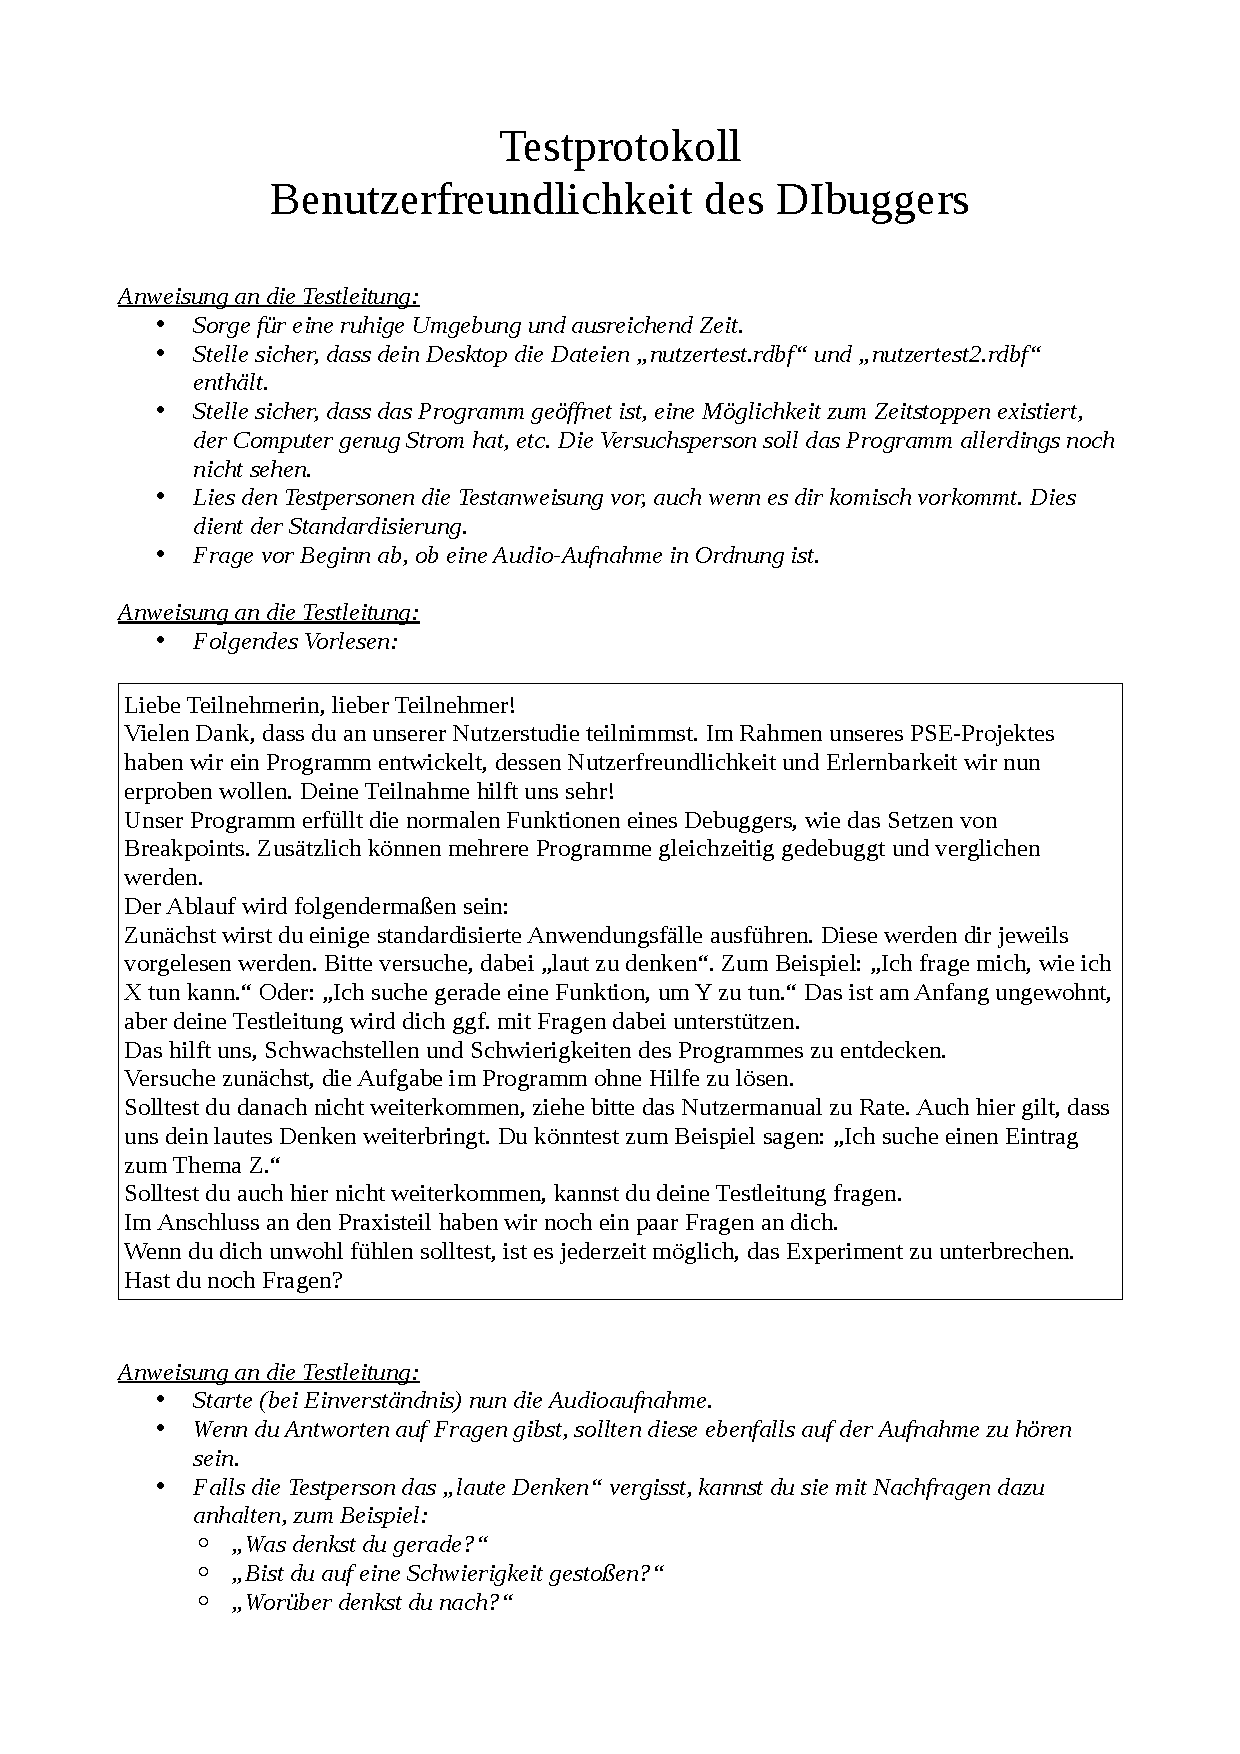
\includepdf[pages={1-},scale=0.75]{UsabilitytestDebugger.pdf}



\end{document}
